\title{CS4221/CS5421}

\subtitle{Tutorial 5: Dependencies, entity-relationship modelling and the Chase}

\author{Mark Meng Huasong}

\institute[National University of Singapore] % (optional, but mostly needed)
{
	School of Computing\\
	National University of Singapore
}

\titlegraphic{
	
\includegraphics[width=2cm]{nus-logo}
}

\date{Week 7, 2022 Spring}

\begin{frame}
	\titlepage
	\begin{tcolorbox}
		\begin{center}
			{\scriptsize \textcolor{red}{All the materials within presentation slides are protected by copyrights.\\
					It is forbidden by NUS to upload these materials to the Internet.}}
		\end{center}
	\end{tcolorbox}
\end{frame}

\section*{Question 1 Entity-relationship Design}

\begin{frame}[fragile]{Question 1 Entity-relationship Design}
Consider the entity-relationship diagram of Figure 1.
\begin{figure}
	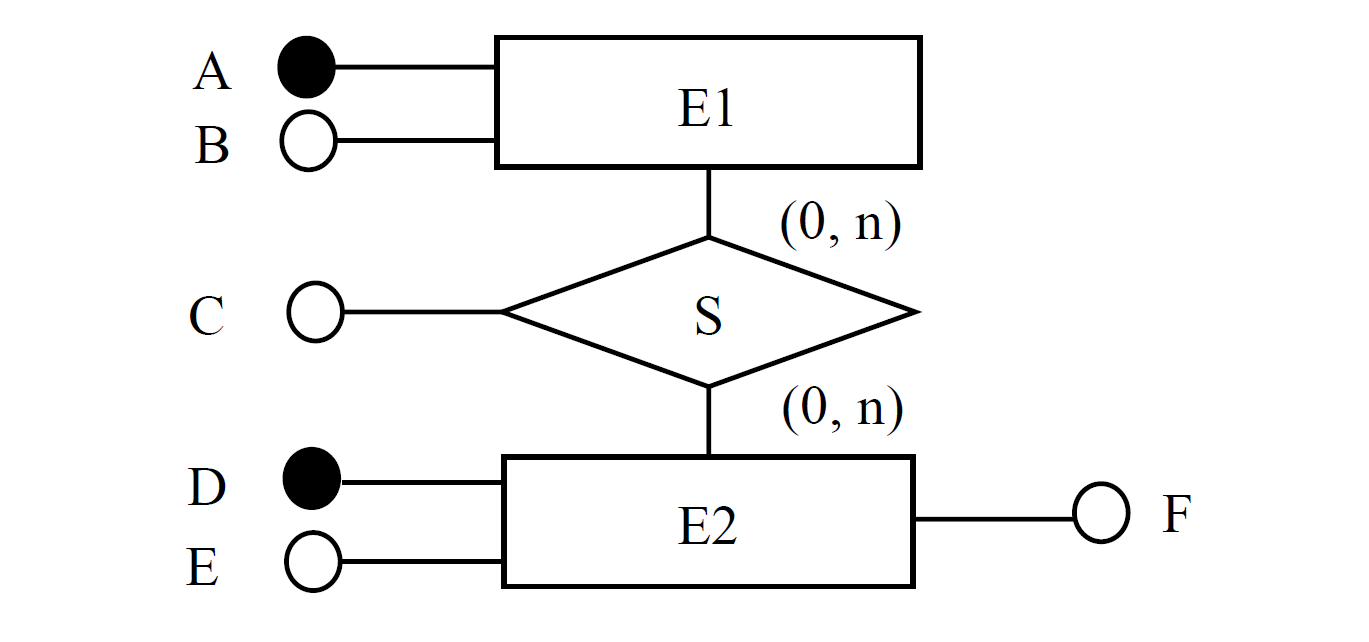
\includegraphics[width=0.75\textwidth, trim=0 0 0 0, clip]{4221-t5/images/q1.png}
\end{figure}
(a) Without other knowledge than that captured by the entity-relationship diagram, what are the \textbf{functional} and \textbf{multi-valued} dependencies?
\end{frame}

\begin{frame}[fragile]{Question 1 (Cont.)}
\textbf{Solution}: The entity-relationship diagram tells us the following functional dependencies.\\ \vspace{5pt}

$\Sigma = \{\{A\}\rightarrow\{B\}, \{D\}\rightarrow\{E,F\}, \{A,D\}\rightarrow\{C\}\}$
\\ \vspace{10pt}

Multi-valued dependencies depend on the translation of this design into tables. The entity-
relationship diagram and its translation will only result in ``not interesting'' multi-valued dependencies, those are trivial or correspond to the table or the functional dependencies.\\ \vspace{5pt}
If we canonically translate this design into three tables, we have
$\{A\} \twoheadrightarrow \{B\}$ and $\{D\}\twoheadrightarrow \{E,F\}$ and many more (none of them being useful for normalisation), for instance.
\end{frame}

\begin{frame}[fragile]{Question 1 (Cont.)}
	
Note that additional knowledge of the application could tell us additional functional and multivalued dependencies not captured by the design.\\ \vspace{5pt}

For instance, we could know that $\{E\}\rightarrow\{F\}$ (which would suggest that the entity-relationship design is probably missing entities and relationships that have been merged too early), which we could use to produce a design in the Boyce-Codd normal by splitting the table $R_3(D,E,F)$ into two tables $R_{3.1}=(\underline{D},E)$ and $R_{3.2}=(\underline{E},F)$.\\ \vspace{5pt}

For instance, we could know that $\{E\}\twoheadrightarrow\{F\}$, which we could use to produce a design in the fifth normal by splitting the table $R_3(D,E,F)$ into two tables $R_{3.1}=(\underline{D},E)$ and $R_{3.2}=(\underline{E,F})$.	
\end{frame}

\section*{Question 2 MVD \& Chase}

\begin{frame}[fragile]{Question 2 MVD}
Consider the relational schema $R = \{A,B,C,D,E\}$ with the following set of functional and multi-valued dependencies.\\ \vspace{5pt}

$\Sigma=\{\{C\}\rightarrow\{A\}, \{D\}\rightarrow\{D,B\}, \{B\}\rightarrow\{E\},\{E\}\twoheadrightarrow\{A,D\},\{A,B,D\}\rightarrow\{A,B,C,D\},\{B\}\rightarrow\{D\}\}$\\ \vspace{5pt}

(a) Prove that $\{E\}\rightarrow\{D\}$ using the Armstrong and multi-valued dependencies axioms.\\ \vspace{5pt}

\end{frame}
\begin{frame}[fragile]{Question 2 MVD (Cont.)}
	\textbf{\underline{Quick Recap:}}\\\vspace{20pt}
	\begin{small}
	\textbf{\textit{Complementation}} $\left( X\twoheadrightarrow Y \right) \Longrightarrow \left( X\twoheadrightarrow R-X-Y \right) $
	 \\\vspace{5pt}
	\textbf{\textit{Augmentation}} $\left( \left( X\twoheadrightarrow Y \right) \land \left( V\subset W \right) \right) \Longrightarrow \left( X\cup W\twoheadrightarrow Y\cup V \right) $
	\\\vspace{5pt}
	\textbf{\textit{Transitivity}} $\left( \left( X\twoheadrightarrow Y \right) \land \left( Y\twoheadrightarrow Z \right) \right) \Longrightarrow \left( X\twoheadrightarrow Z-Y \right) 
	$\\\vspace{5pt}
	\textbf{\textit{Replication/Promotion}} $\left( X\rightarrow Y \right) \Longrightarrow \left( X\twoheadrightarrow Y \right) $ \\\vspace{5pt}
	\textbf{\textit{Coalescence}} $\left( \left( X\twoheadrightarrow Y \right) \land \left( W\rightarrow Z \right) \land \left( Z\subset Y \right) \land \left( W\cap Y=\emptyset \right) \right) \Longrightarrow \left( X\rightarrow Z \right) $ \\\vspace{5pt}
	\textbf{\textit{Union}} $\left( \left( X\twoheadrightarrow Y \right) \land \left( X\twoheadrightarrow Z \right) \right) \Longrightarrow \left( X\twoheadrightarrow Y\cup Z \right) $ \\\vspace{5pt}
	\textbf{\textit{Intersection}} $\left( \left( X\twoheadrightarrow Y \right) \land \left( X\twoheadrightarrow Z \right) \right) \Longrightarrow \left( X\twoheadrightarrow Y\cap Z \right) $ \\\vspace{5pt}
	\textbf{\textit{Difference}} $\left( \left( X\twoheadrightarrow Y \right) \land \left( X\twoheadrightarrow Z \right) \right) \Longrightarrow \left( X\twoheadrightarrow Y-Z \right) $ \\\vspace{5pt}
	\end{small}

\end{frame}
\begin{frame}[fragile]{Question 2 MVD (Cont.)}
\textbf{Solution:}\\ \vspace{5pt}
1. We know that $\{E\}\twoheadrightarrow\{A,D\}$.\\ \vspace{2pt}
2. We know that $\{B\}\rightarrow\{D\}$.\\\vspace{2pt}
3. We see that $\{D\}\subset\{A,D\}$.\\\vspace{2pt}
4. We see that $\{B\}\cap \{A,D\}=\emptyset$\\\vspace{2pt}
5. Therefore $\{E\}\rightarrow\{D\}$ by Coalescence of (1), (2), (3) and (4).\\\vspace{2pt}
\hfill Q.E.D.\\\vspace{10pt}
Try the same question with the Chase (answer not provided).
\end{frame}

\begin{frame}[fragile]{Question 3 Chase}
Consider the relation $R(A,B,C,D,E,G)$ with the following set, $F$, of functional and multi-valued dependencies.\\ \vspace{5pt}
	
$F=\{\{A,B\}\rightarrow\{C\}, \{A,B\}\twoheadrightarrow\{E\},\{C,D\}\twoheadrightarrow\{A,B\}\}$\\ \vspace{5pt}
	
Prove that the decomposition of $R$ into $R_1(A,B,C,D,G)$ and $R_2(C,D,E)$ is lossless using the Chase algorithm (as shown in the lecture).\\ \vspace{5pt}

\textbf{\textcolor{blue}{How to solve this question?}}\\\vspace{5pt}
\textcolor{blue}{Recall the lecture note ``\emph{Testing if a decomposition is lossless}''.
We first analyze the decomposition to find out what is the $X$ of ``$R=X\cup Y\cup Z$''. We have $X=\{C,D\}$.\\\vspace{2pt}
Then we need to use the Chase method to chase $\{C,D\}\twoheadrightarrow\{E\}$ ({\small or $\{C,D\}\twoheadrightarrow\{A,B,G\}$ equivalently, according to Complementation rule of Armstrong Axiom}).}\\\vspace{5pt}

\textcolor{blue}{Now the question becomes:\\
$\{\{A,B\}\rightarrow\{C\}, \{A,B\}\twoheadrightarrow\{E\},\{C,D\}\twoheadrightarrow\{A,B\}\} \models \{C,D\}\twoheadrightarrow\{E\}$?.}
\end{frame}

\begin{frame}[fragile]{Question 3 (Cont.)}	
\textbf{Solution:}\\ \vspace{2pt}
1. Initial table.\\
\begin{figure}
	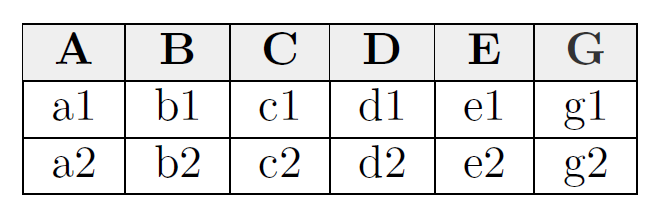
\includegraphics[width=0.4\textwidth, trim=0 0 0 0, clip]{4221-t5/images/3-1.png}
\end{figure}

2. We want to chase $\{C,D\} \twoheadrightarrow \{E\}$, make $C$ and $D$ values the same.\\
\begin{figure}
	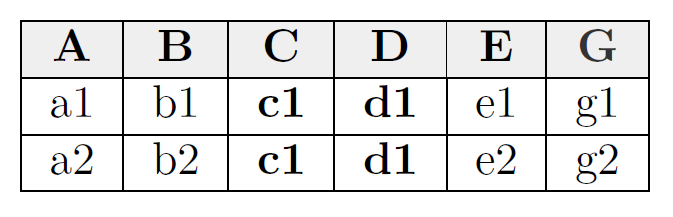
\includegraphics[width=0.4\textwidth, trim=0 0 0 0, clip]{4221-t5/images/3-2.png}
\end{figure}

\end{frame}

\begin{frame}[fragile]{Question 3 (Cont.)}
3. Apply $\{C,D\} \twoheadrightarrow \{A,B\}$ by copying two tuples that have the same $C$ and $D$ values but swapping their $A$ and $B$ values.\\\vspace{10pt}

\textcolor{blue}{{\small Below are cited from the ``Chasing the Chase'' part of the lecture note:\\\vspace{5pt}
\textit{For each multi-valued dependency $Z\twoheadrightarrow V\in\Sigma$, if there are 2 tuples in the table with the \textbf{SAME $Z$-value}, then add two new tuples with \textbf{all the same values and except} for their $V$-values that are \textbf{SWAPPED}.}}}

\begin{figure}
	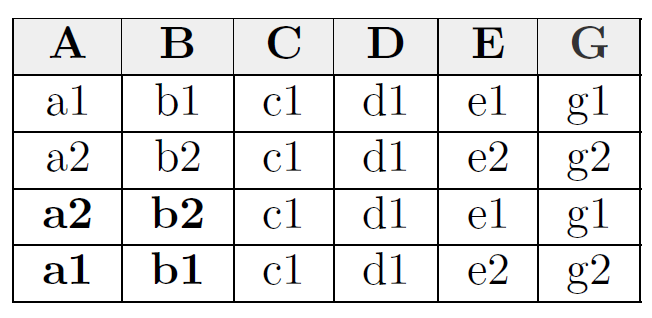
\includegraphics[width=0.4\textwidth, trim=0 0 0 0, clip]{4221-t5/images/3-3.png}
\end{figure}

\end{frame}


\begin{frame}[fragile]{Question 3 (Cont.)}
4. Apply $\{A,B\} \twoheadrightarrow \{E\}$ by copying two tuples that have the same $A$ and $B$ values but swapping their $A$ and $E$ values.\\
\begin{figure}
	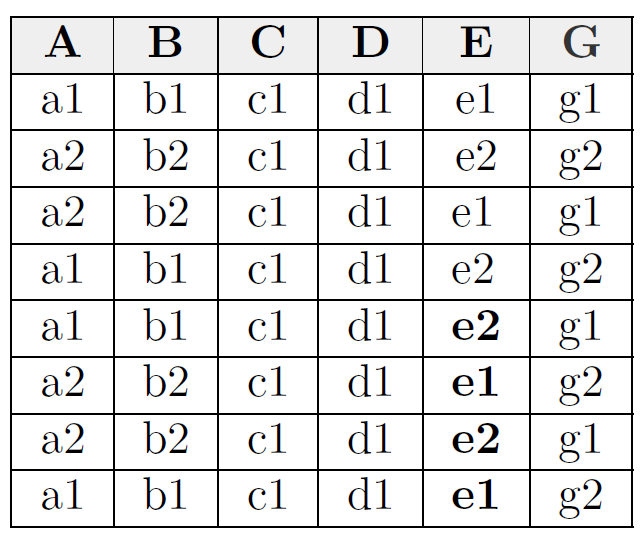
\includegraphics[width=0.4\textwidth, trim=0 0 0 0, clip]{4221-t5/images/3-4.png}
\end{figure}
\end{frame}


\begin{frame}[fragile]{Question 3 (Cont.)}
5. Applying $\{A,B\} \rightarrow \{C\}$ do not change the table.\\\vspace{5pt}
\textcolor{blue}{{\small \textit{Because we cannot find for any two tuples $\{a1,b1,c1,...\}$ and $\{a2,b2,c2,...\}$ s.t. $\{a1,b1\}=\{a2,b2\}$ but $c1 \ne c2$}.}}\\\vspace{5pt}

6. Sort the table and proved that $\{C,D\}\twoheadrightarrow\{E\}$ 
	\begin{figure}
		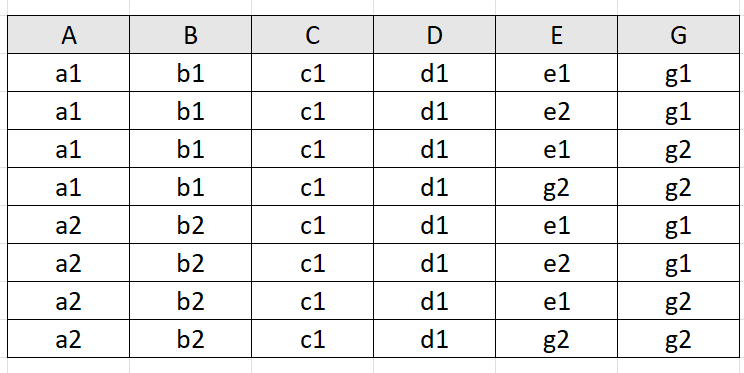
\includegraphics[width=0.6\textwidth, trim=0 0 0 0, clip]{4221-t5/images/3-6a.png}
	\end{figure}

\textcolor{red}{{\small \textit{Refer to the lecture slides ``Dependencies'' page 77 for the definition of a MVD.}}}\\\vspace{5pt}
OR \textcolor{blue}{{\small \textit{Because we cannot find any counterexample.}}}
\textcolor{red}{{\small \textit{Refer to the lecture slides ``The Chase'' page 18: The Chase always builds a counter example if it exists and does not if it does not exists.}}}\\\vspace{10pt}


	\hfill Q.E.D
\end{frame}


\begin{frame}[fragile]{Question 4 Chase}
	Consider the relation $R(A,B,C,D,E,F,G)$ with the following set, $\Sigma$, of functional dependencies.\\ \vspace{5pt}
	
	$\Sigma=\{\{A,B\}\rightarrow\{C\},\{C\}\rightarrow\{D,E\},\{E\}\rightarrow\{D\},\{F\}\rightarrow\{G\}\}$\\ \vspace{5pt}
	
	Prove that the decomposition of $R$ into $R_1(A,B,C,D,E)$ and $R_2(A,B,F,G)$ is lossless using the Chase algorithm (as shown in the lecture).\\ \vspace{5pt}
	
	\textbf{Solution:}\\ \vspace{2pt}
	1. Initial table.\\
	\begin{figure}
		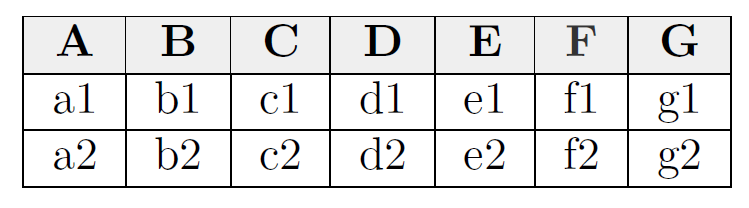
\includegraphics[width=0.4\textwidth, trim=0 0 0 0, clip]{4221-t5/images/4-1.png}
	\end{figure}
	
	2. We want to chase $\{A,B\} \twoheadrightarrow \{C,D,E\}$, make $A$ and $B$ values the same.\\
	\begin{figure}
		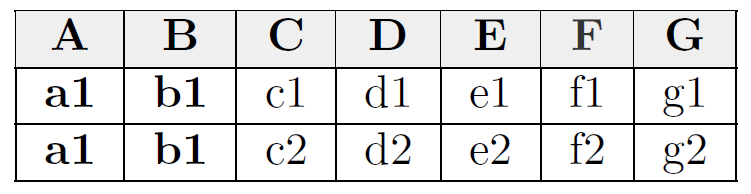
\includegraphics[width=0.4\textwidth, trim=0 0 0 0, clip]{4221-t5/images/4-2.png}
	\end{figure}	
\end{frame}

\begin{frame}[fragile]{Question 4 (Cont.)}
	3. Apply $\{A,B\} \rightarrow \{C\}$, make $C$ with the same $A$ and $B$ values the same.\\
	\begin{figure}
		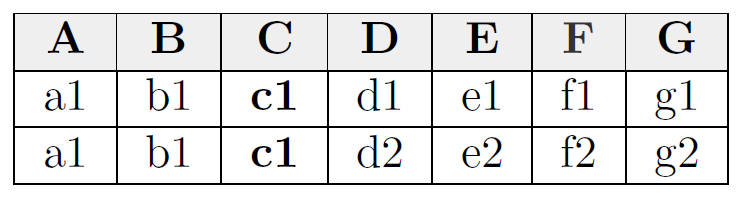
\includegraphics[width=0.4\textwidth, trim=0 0 0 0, clip]{4221-t5/images/4-3.png}
	\end{figure}
	
	4. Apply $\{C\} \rightarrow \{D,E\}$, make $D$ and $E$ with the same $C$ values the same.\\
	\begin{figure}
		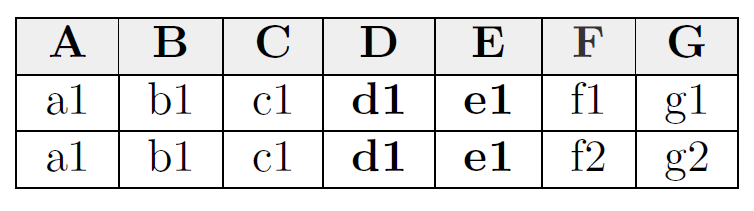
\includegraphics[width=0.4\textwidth, trim=0 0 0 0, clip]{4221-t5/images/4-4.png}
	\end{figure}

	5. Applying $\{E\} \rightarrow \{D\}$ does not change the table.\\\vspace{5pt}
	6. Applying $\{F\} \rightarrow \{G\}$ does not change the table.\\\vspace{5pt}
	7. Proved that $\{A,B\} \twoheadrightarrow \{C,D,E\}.$\\
	\hfill Q.E.D
	
\end{frame}


\begin{frame}[fragile]{Question 5 Chase with the Distinguished Attributes}
	Consider the relation $R(A,B,C,D,E)$ with the following set, $F$, of functional dependencies.\\ \vspace{5pt}
	
	$\Sigma=\{\{A\}\rightarrow\{B,C\}, \{B\}\rightarrow\{A\},\{C\}\rightarrow\{D\}\}$\\ \vspace{5pt}
	
	Check whether the decomposition of $R$ into $R_1(A,E)$, $R_2(C,D)$ and $R_3(A,B,C)$ is lossless using the Chase algorithm with the distinguished attributes.\\ \vspace{5pt}
	
	\textbf{Solution:}\\ \vspace{2pt}
	1. Initial table.\\
	\begin{figure}
		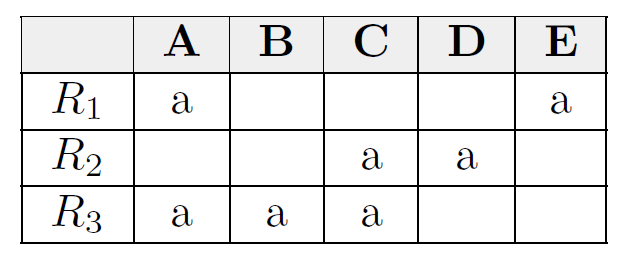
\includegraphics[width=0.3\textwidth, trim=0 0 0 0, clip]{4221-t5/images/5-1.png}
	\end{figure}
	
	2. Apply $\{A\} \rightarrow \{B,C\}$.\\
	\begin{figure}
		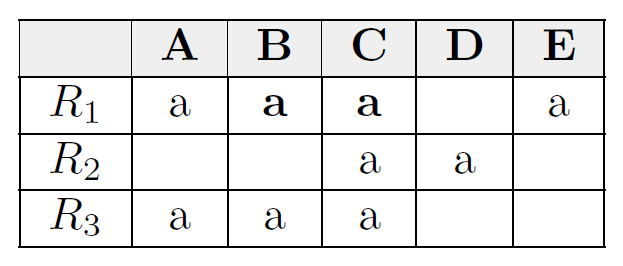
\includegraphics[width=0.3\textwidth, trim=0 0 0 0, clip]{4221-t5/images/5-2.png}
	\end{figure}
	
\end{frame}
\begin{frame}[fragile]{Question 5 (Cont.)}
	
	3. Applying $\{B\} \rightarrow \{A\}$ does not change the table.\\
	4. Apply $\{C\} \rightarrow \{D\}$.\\
	\begin{figure}
		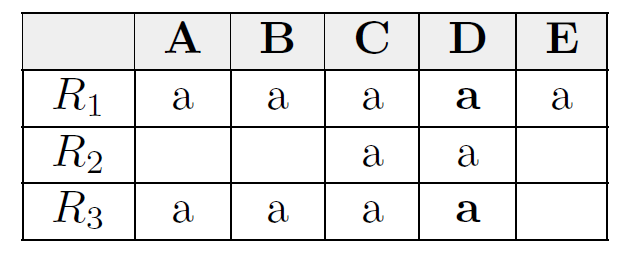
\includegraphics[width=0.3\textwidth, trim=0 0 0 0, clip]{4221-t5/images/5-4.png}
	\end{figure}

	5. $R_1$ has distinguished variables in all of the columns, therefore the decomposition is lossless.\\
	\hfill Q.E.D
\end{frame}

\section*{Extra Practice}
\begin{frame}[fragile]{Extra Practice (A): MVD \& Chase}
\underline{Q2 Revisit}: consider the relational schema $R = \{A,B,C,D,E\}$ with the following set of functional and multi-valued dependencies.\\ \vspace{5pt}

$\Sigma=\{\{C\}\rightarrow\{A\}, \{D\}\rightarrow\{D,B\}, \{B\}\rightarrow\{E\},\{E\}\twoheadrightarrow\{A,D\},\{A,B,D\}\rightarrow\{A,B,C,D\},\{B\}\rightarrow\{D\}\}$\\ \vspace{5pt}

Prove that $\{E\}\rightarrow\{D\}$ using the \textbf{Chase algorithm}.\\ \vspace{25pt}

\underline{Q3-4 Revisit}: prove them by using Armstrong axiom.\\ 

\end{frame}

\begin{frame}[fragile]{Extra Practice (B): ER Participation vs. Logical Design}
Can you spot the difference among the 4 cases below? Can you explain what they look like in the logical design? Can you give an example from the real world for each case?\\ \vspace{4pt}
	
\begin{figure}
	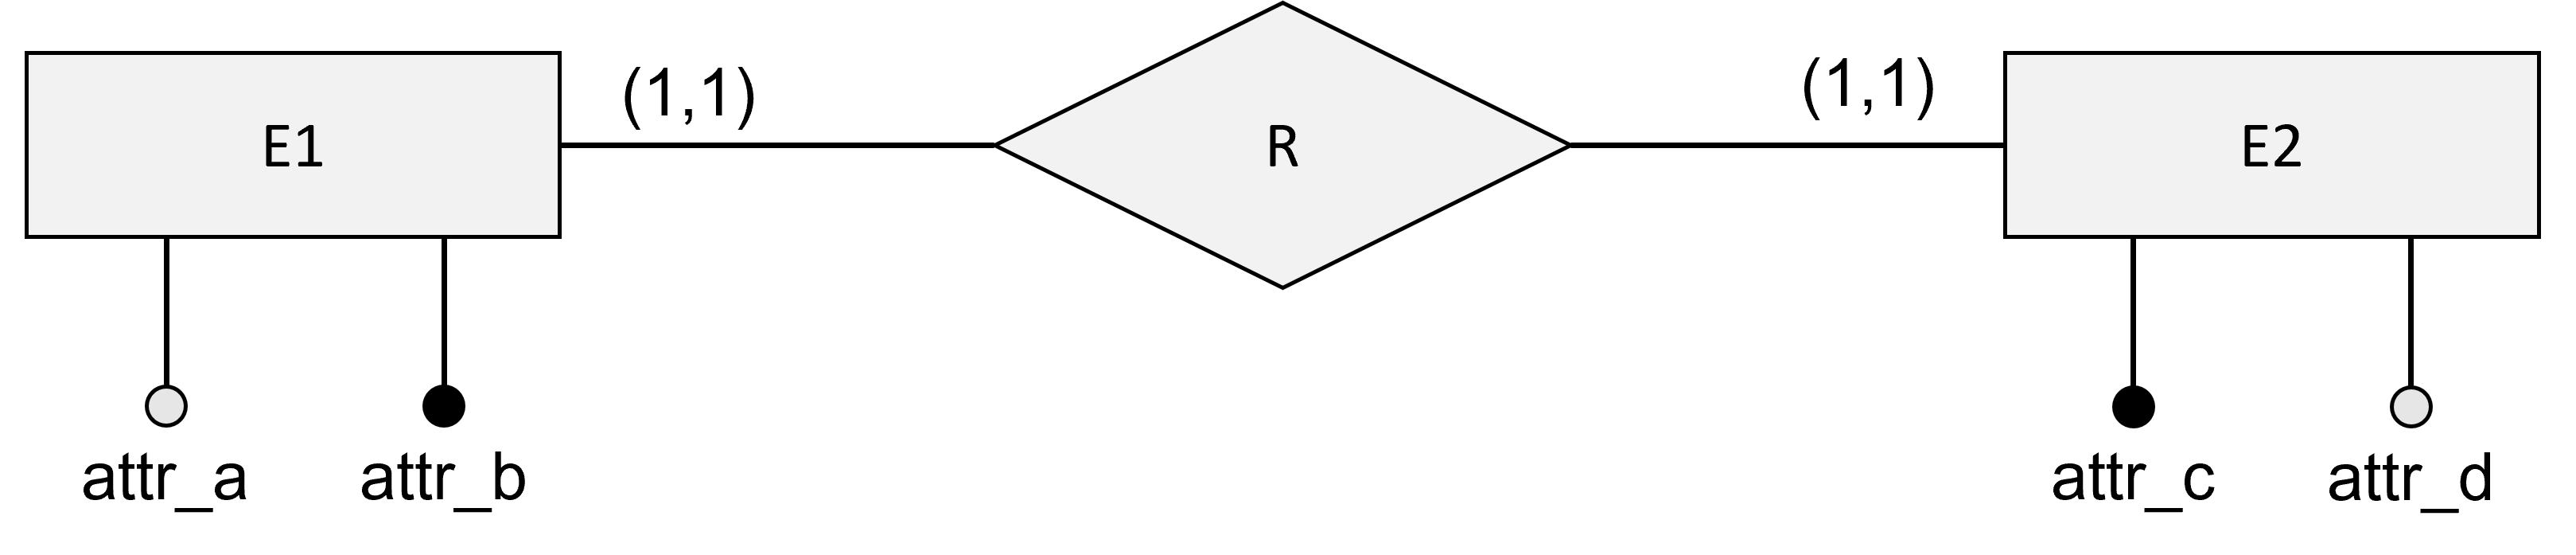
\includegraphics[width=0.65\textwidth, trim=0 0 0 0, clip]{t4/images/case1.png}
	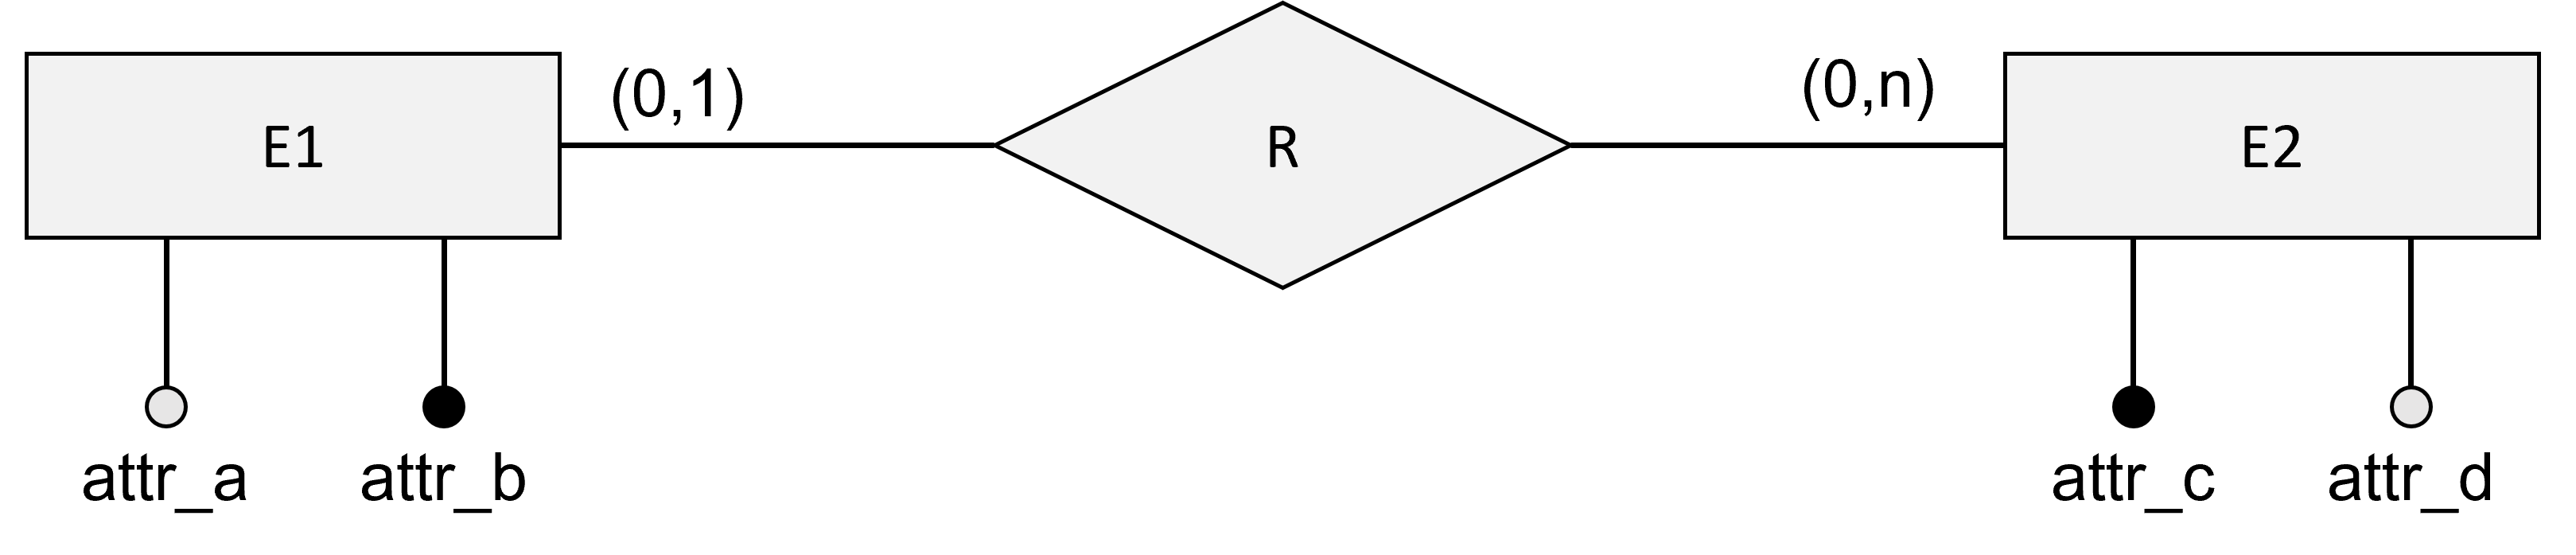
\includegraphics[width=0.65\textwidth, trim=0 0 0 0, clip]{t4/images/case2.png}
	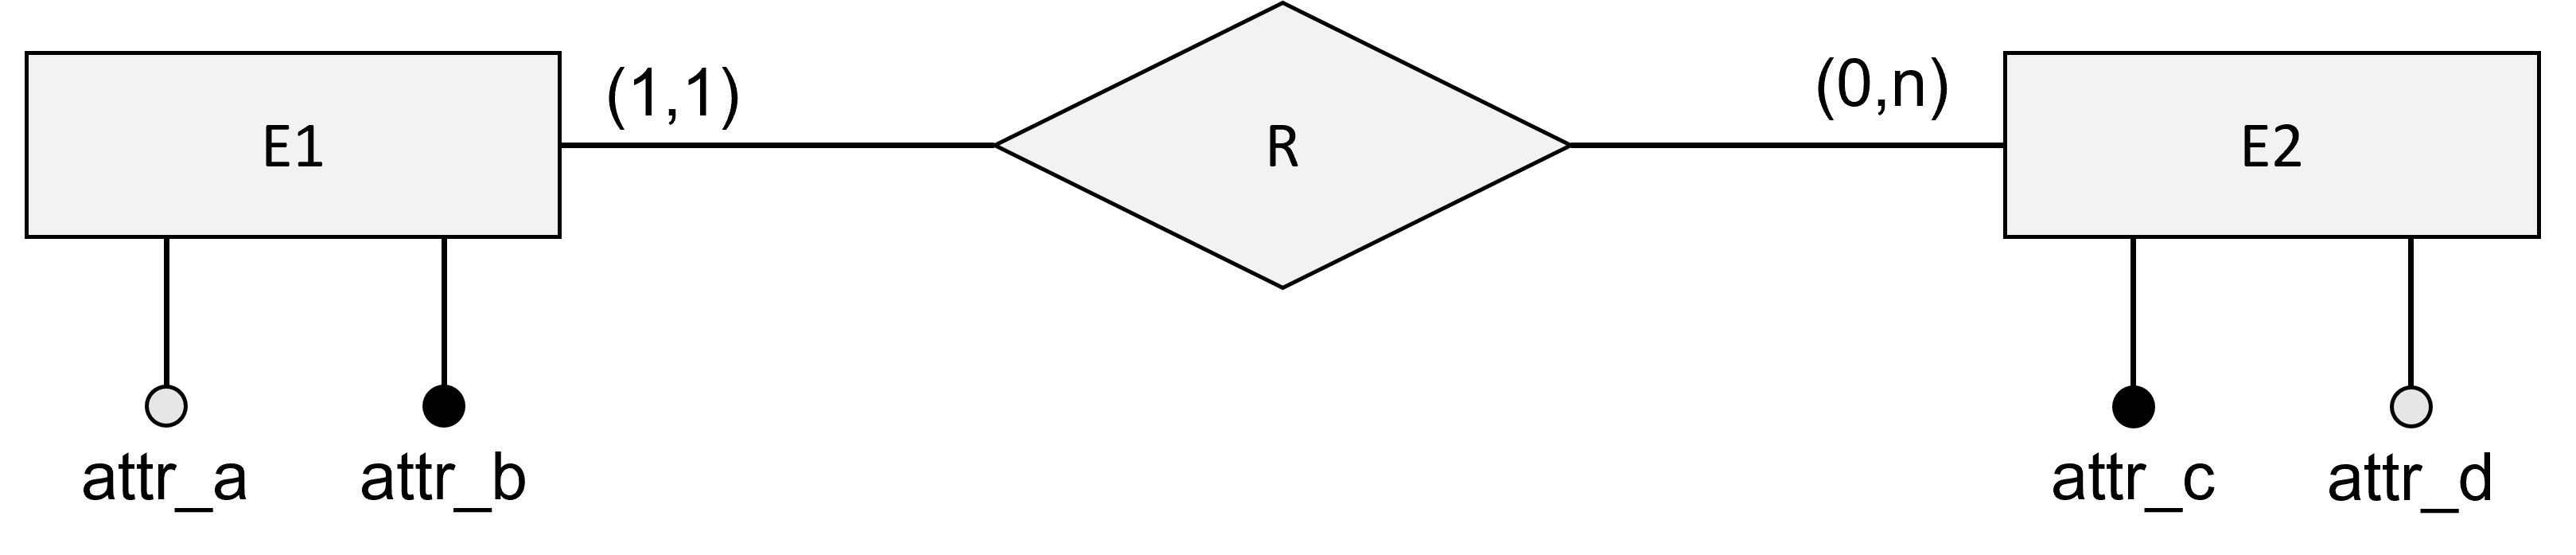
\includegraphics[width=0.65\textwidth, trim=0 0 0 0, clip]{t4/images/case3.png}
	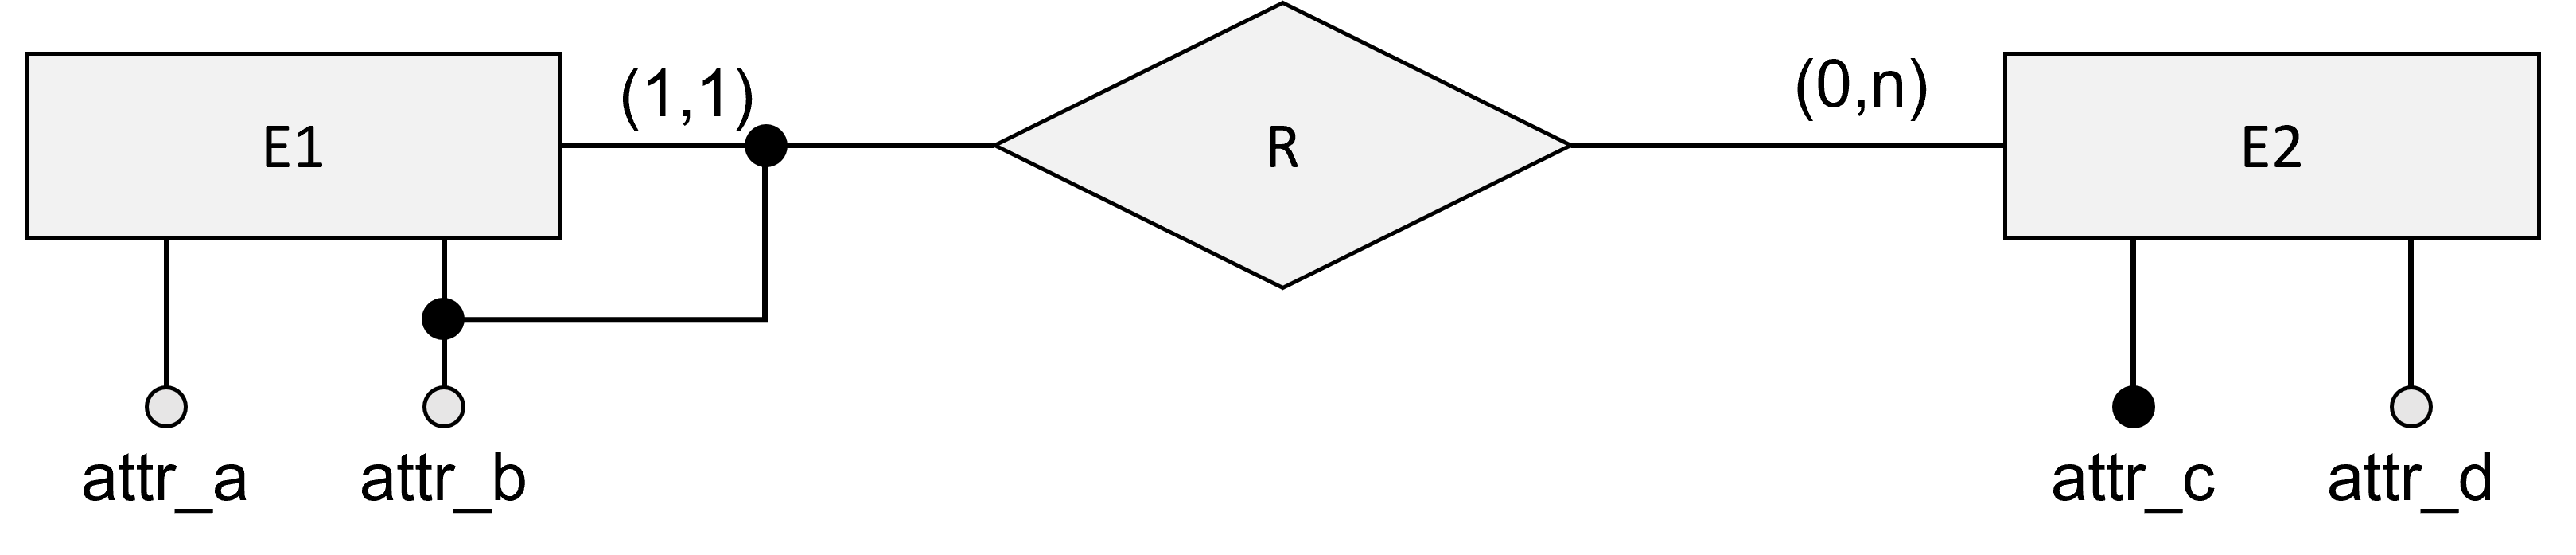
\includegraphics[width=0.65\textwidth, trim=0 0 0 0, clip]{t4/images/case4.png}
\end{figure}
\end{frame}

\begin{frame}[fragile]{Extra Practice (Case 1)}
\begin{figure}
	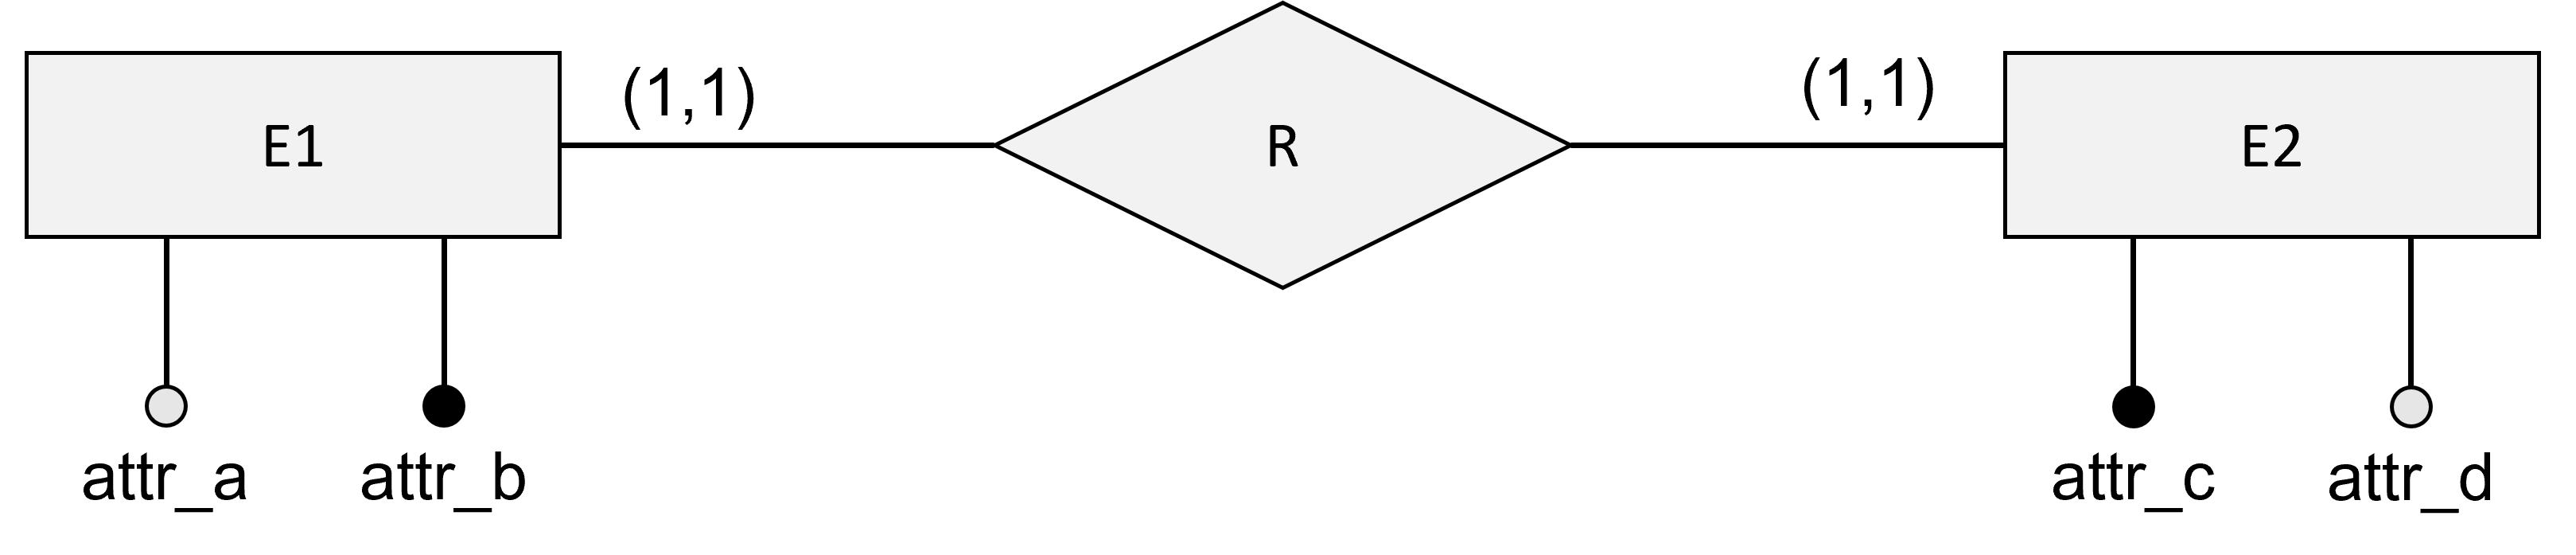
\includegraphics[width=0.65\textwidth, trim=0 0 0 0, clip]{t4/images/case1.png}
\end{figure}

\begin{columns}
\column{0.5\textwidth}
\begin{figure}
	\centering
	E1 as \textbf{political\_party},\\E2 as \textbf{secretary\_general},\\R as \textbf{led\_by}\vspace{10pt}
	\scriptsize
	\begin{tikzpicture}[ele/.style={fill=black,minimum size=1pt,circle}, node distance=5pt]
		\node[ele,label=left:People's Action] (a1) {};    
		\node[ele,label=left:Workers (S'pore)] (a2) [below=of a1] {};    
		\node[ele,label=left:Progress Singapore] (a3) [below=of a2] {};
		\node[ele,label=left:Reform (S'pore)] (a4) [below=of a3]  {};
		
		\node[ele,,label=right:Lee Hsien Loong] (b1) [right=of a1,xshift=15pt] {};
		\node[ele,,label=right:Francis Yuen] (b2) [below=of b1] {};
		\node[ele,,label=right:Pritam Singh] (b3) [below=of b2] {};
		\node[ele,,label=right:Kenneth Jeyaretnam] (b4) [below=of b3] {};
		
		%\node[draw,fit= (a1) (a2) (a3) (a4),minimum width=2cm] {} ;
		%\node[draw,fit= (b1) (b2) (b3) (b4),minimum width=2cm] {} ;  
		\draw[-,thick,shorten <=2pt,shorten >=2pt] (a1) -- (b1);
		\draw[-,thick,shorten <=2pt,shorten >=2] (a2) -- (b3);
		\draw[-,thick,shorten <=2pt,shorten >=2] (a3) -- (b2);
		\draw[-,thick,shorten <=2pt,shorten >=2] (a4) -- (b4);
	\end{tikzpicture}
\end{figure}

\column{0.01\textwidth}
\column{0.47\textwidth}
\underline{\textbf{Table E1}}: \\\faIcon{key} name,\\ secretary\_general \\\vspace{5pt}
\textit{or \underline{alternatively}, we define}\\\vspace{5pt}
\underline{\textbf{Table E2}}:\\\faIcon{key} name\\ leading\_party,
\end{columns}
\end{frame}

\begin{frame}[fragile]{Extra Practice (Case 2)}
	\begin{figure}
		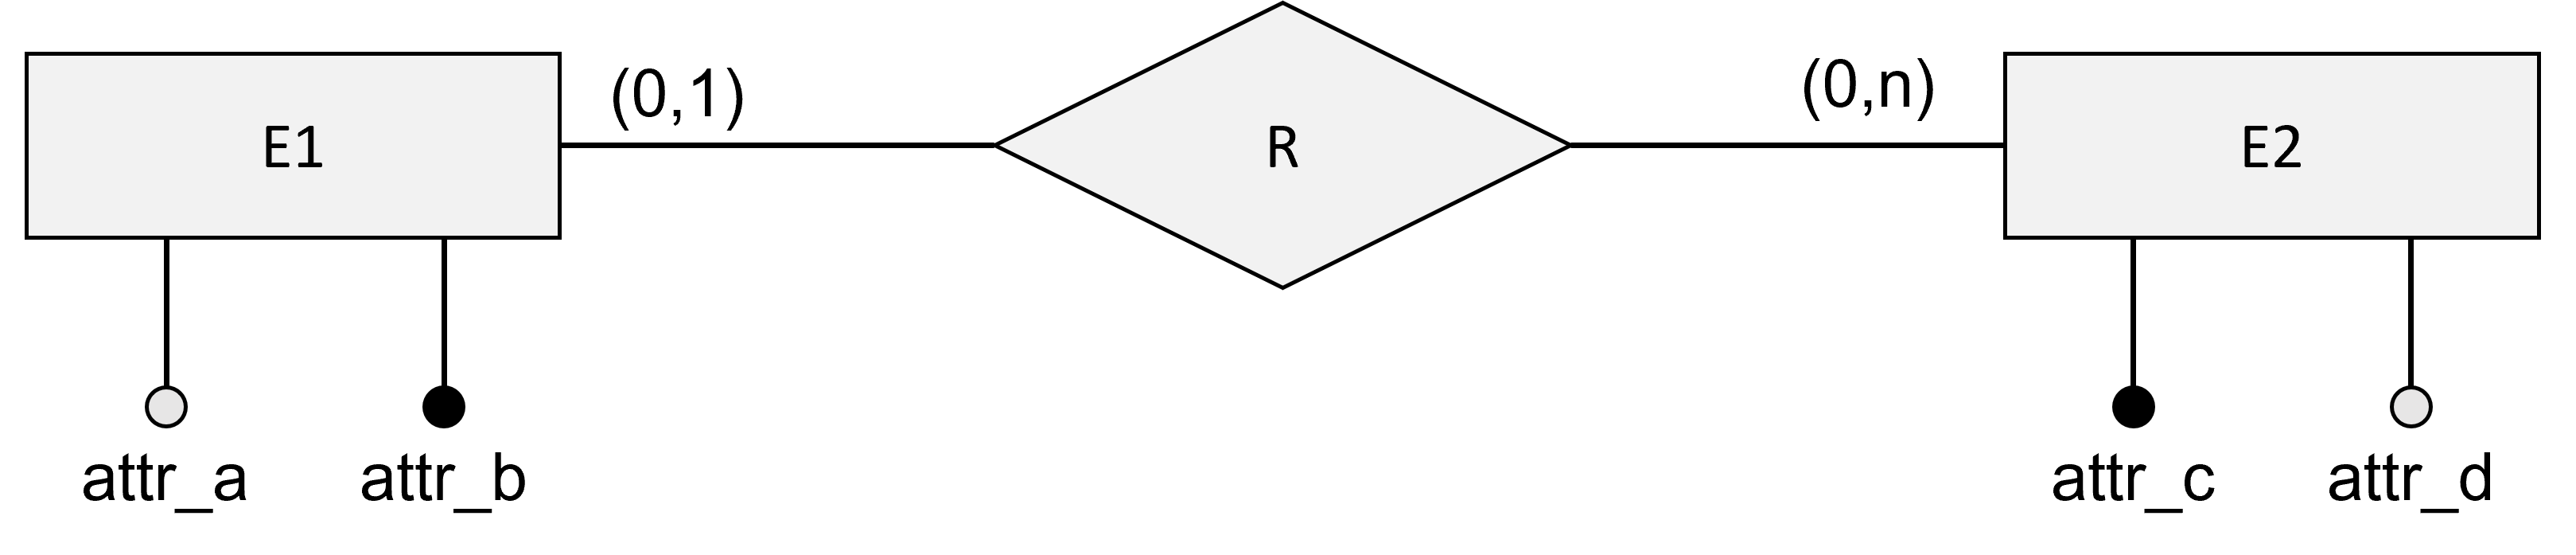
\includegraphics[width=0.58\textwidth, trim=0 0 0 0, clip]{t4/images/case2.png}
	\end{figure}
	
	\begin{columns}
		\column{0.52\textwidth}
		\begin{figure}
			\centering
			E1 as \textbf{parliament\_member},\\E2 as \textbf{political\_party},\\R as \textbf{belongs\_to}\vspace{10pt}
			\scriptsize
			\begin{tikzpicture}[ele/.style={fill=black,minimum size=1pt,circle}, node distance=5pt]
				\node[ele,label=left:Pritam Singh] (a1) {};    
				\node[ele,label=left:Lee Hsien Loong] (a2) [below=of a1] {};    
				\node[ele,label=left:K Shanmugam] (a3) [below=of a2] {};
				\node[ele,label=left:Hazel Poa] (a4) [below=of a3]  {};
				\node[ele,label=left:Lawrence Wong] (a5) [below=of a4]  {};
				\node[ele,label=left:Hoon Hian Teck] (a6) [below=of a5]  {};
				\node[ele,label=left:Jamus Lin] (a7) [below=of a6]  {};
				\node[ele,label=left:Chan Chun Sing] (a8) [below=of a7]  {};
				
				\node[ele,,label=right:People's Action] (b1) [right=of a3,xshift=30pt] {};
				\node[ele,,label=right:Workers (S'pore)] (b2) [below=of b1] {};
				\node[ele,,label=right:Reform (S'pore)] (b3) [below=of b2] {};
				\node[ele,,label=right:Progress S'pore] (b4) [below=of b3] {};
				
				%\node[draw,fit= (a1) (a2) (a3) (a4),minimum width=2cm] {} ;
				%\node[draw,fit= (b1) (b2) (b3) (b4),minimum width=2cm] {} ;  
				\draw[-,thick,shorten <=2pt,shorten >=2pt] (a1) -- (b2);  
				\draw[-,thick,shorten <=2pt,shorten >=2pt] (a7) -- (b2);
				\draw[-,thick,shorten <=2pt,shorten >=2] (a2) -- (b1);
				\draw[-,thick,shorten <=2pt,shorten >=2] (a3) -- (b1);
				\draw[-,thick,shorten <=2pt,shorten >=2] (a5) -- (b1);
				\draw[-,thick,shorten <=2pt,shorten >=2] (a8) -- (b1);
				\draw[-,thick,shorten <=2pt,shorten >=2] (a4) -- (b4);
			\end{tikzpicture}
		\end{figure}
		
		\column{0.48\textwidth}
		\underline{\textbf{Table E1}}: \\\faIcon{key} name \\\vspace{5pt}
		\underline{\textbf{Table E2}}: \\\faIcon{key} name \\\vspace{5pt}
		\underline{\textbf{Table R}}: \\\faIcon{key}~\faIcon{arrow-right} member\_name (E1.name), \\
		\faIcon{arrow-right} affiliation\_party (E2.name)
		\vspace{5pt}
	\end{columns}
\end{frame}


\begin{frame}[fragile]{Extra Practice (Case 3)}
	\begin{figure}
		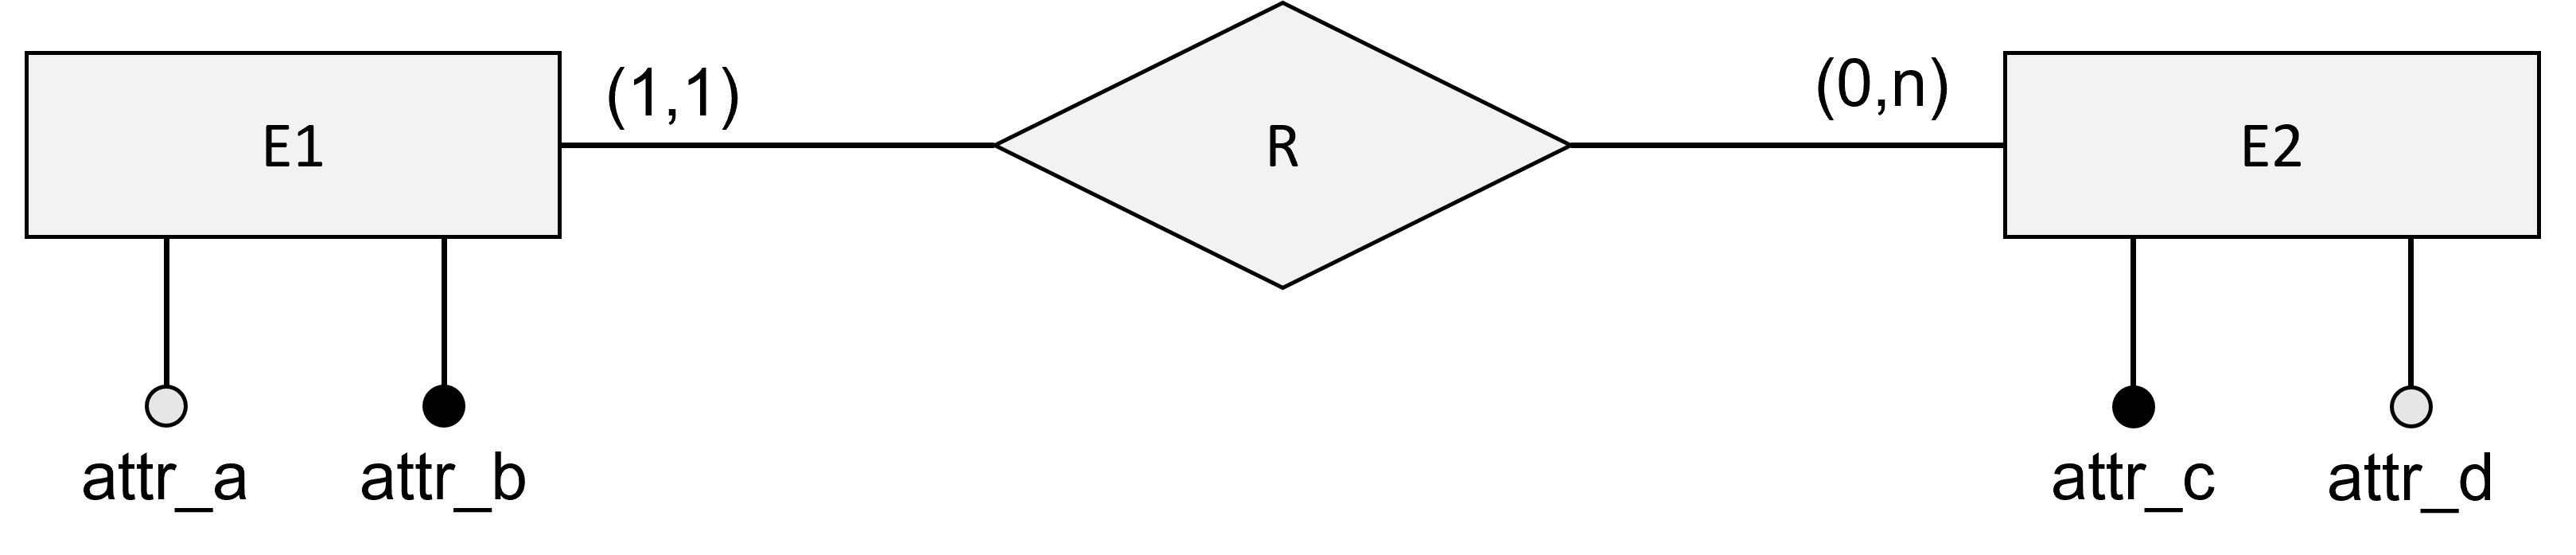
\includegraphics[width=0.65\textwidth, trim=0 0 0 0, clip]{t4/images/case3.png}
	\end{figure}
	
	\begin{columns}
		\column{0.5\textwidth}
		\begin{figure}
			\centering
			E1 as \textbf{government},\\E2 as \textbf{parliament\_member},\\R as \textbf{head}\vspace{10pt}
			\scriptsize
			\begin{tikzpicture}[ele/.style={fill=black,minimum size=1pt,circle}, node distance=5pt] 
				\node[ele,label=left:Prime Minister Office] (a1) {};    
				\node[ele,label=left:Ministry of Finance] (a2) [below=of a1] {};    
				\node[ele,label=left:Ministry of Law] (a3) [below=of a2] {};
				\node[ele,label=left:Ministry of Home Affairs] (a4) [below=of a3]  {};
				
				\node[ele,label=right:Pritam Singh] (b1) [right=of a1, above=of a1,xshift=25pt] {};
				\node[ele,,label=right:K Shanmugam] (b2) [below=of b1] {};
				\node[ele,,label=right:Lawrence Wong] (b3) [below=of b2] {};
				\node[ele,,label=right:Jamus Lim] (b4) [below=of b3] {};
				\node[ele,,label=right:Lee Hsien Loong] (b5) [below=of b4] {};
				\node[ele,,label=right:Patrick Tay] (b6) [below=of b5] {};
				
				%\node[draw,fit= (a1) (a2) (a3) (a4),minimum width=2cm] {} ;
				%\node[draw,fit= (b1) (b2) (b3) (b4),minimum width=2cm] {} ;  
				\draw[-,thick,shorten <=1pt,shorten >=1pt] (a1) -- (b5);
				\draw[-,thick,shorten <=1pt,shorten >=1] (a2) -- (b3);
				\draw[-,thick,shorten <=1pt,shorten >=1] (a3) -- (b2);
				\draw[-,thick,shorten <=1pt,shorten >=1] (a4) -- (b2);
			\end{tikzpicture}
		\end{figure}
		
		\column{0.42\textwidth}
		
		\underline{\textbf{Table E1}}: \\\faIcon{key} government\_name\\ \faIcon{arrow-right} name (E2.name) \\\vspace{5pt}
		\underline{\textbf{Table E2}}: \\\faIcon{key} name
	\end{columns}
\end{frame}


\begin{frame}[fragile]{Extra Practice (Case 4)}
	\begin{figure}
		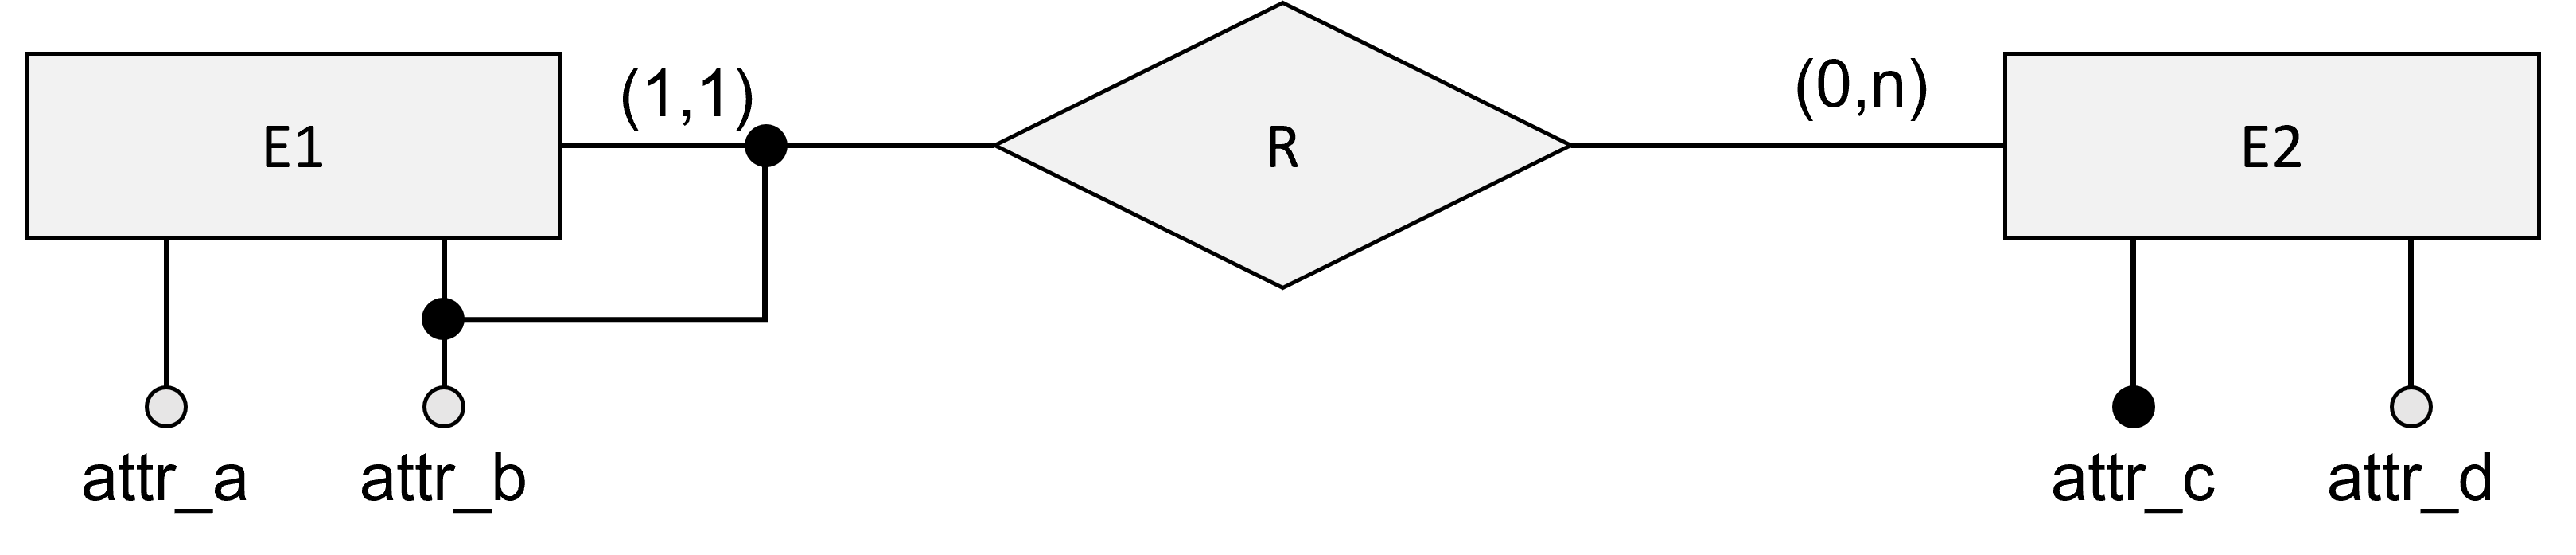
\includegraphics[width=0.65\textwidth, trim=0 0 0 0, clip]{t4/images/case4.png}
	\end{figure}
	
	\begin{columns}
		\column{0.5\textwidth}
		\begin{figure}
			\centering
			E1 as \textbf{party},\\E2 as \textbf{country},\\R as \textbf{belongs\_to}\vspace{10pt}
			\scriptsize
			\begin{tikzpicture}[ele/.style={fill=black,minimum size=1pt,circle}, node distance=5pt]
				\node[ele,label=left:People's Action] (a1) {};    
				\node[ele,label=left:Workers (S'pore)] (a2) [below=of a1] {}; 
				\node[ele,label=left:Workers (India)] (a3) [below=of a2] {};
				\node[ele,label=left:Workers (Hungary)] (a4) [below=of a3] {};     
				\node[ele,label=left:Progress Singapore] (a5) [below=of a4] {};
				\node[ele,label=left:Reform (S'pore)] (a6) [below=of a5]  {};
				\node[ele,label=left:Reform (Canada)] (a7) [below=of a6]  {};
				\node[ele,label=left:Reform (USA)] (a8) [below=of a7]  {};
				
				\node[ele,,label=right:Hungary] (b1) [right=of a2,xshift=25pt] {};
				\node[ele,,label=right:Singapore] (b2) [below=of b1] {};
				\node[ele,,label=right:Canada] (b3) [below=of b2] {};
				\node[ele,,label=right:India] (b4) [below=of b3] {};
				\node[ele,,label=right:Malaysia] (b5) [below=of b4] {};
				\node[ele,,label=right:USA] (b6) [below=of b5] {};
				
				%\node[draw,fit= (a1) (a2) (a3) (a4),minimum width=2cm] {} ;
				%\node[draw,fit= (b1) (b2) (b3) (b4),minimum width=2cm] {} ;  
				\draw[-,thick,shorten <=2pt,shorten >=2pt] (a1) -- (b2);
				\draw[-,thick,shorten <=2pt,shorten >=2] (a2) -- (b2);
				\draw[-,thick,shorten <=2pt,shorten >=2] (a5) -- (b2);
				\draw[-,thick,shorten <=2pt,shorten >=2] (a6) -- (b2);
				\draw[-,thick,shorten <=2pt,shorten >=2] (a3) -- (b4);
				\draw[-,thick,shorten <=2pt,shorten >=2] (a4) -- (b1);
				\draw[-,thick,shorten <=2pt,shorten >=2] (a7) -- (b3);
				\draw[-,thick,shorten <=2pt,shorten >=2] (a8) -- (b6);
			\end{tikzpicture}
		\end{figure}
		
		\column{0.02\textwidth}
		\column{0.45\textwidth}
	
		\underline{\textbf{Table E1}}: \\\faIcon{key} party\_name\\ \faIcon{key}~\faIcon{arrow-right} country (E2.name) \\\vspace{5pt}
		\underline{\textbf{Table E2}}: \\\faIcon{key} name
	\end{columns}
\end{frame}
	
\begin{frame}{}
	\centering  
	For any further question, please feel free to email me:\vspace{10pt}
	
	huasong.meng@u.nus.edu \vspace{20pt}
	
	\begin{tcolorbox}
		\begin{center}
			\textcolor{red}{Cases in the extra practice are contributed by our students.\\\vspace{5pt}Copyright 2022 Mark H. Meng. All rights reserved.}
		\end{center}
	\end{tcolorbox}
\end{frame}